%%%%%%%%%%%%%%%%%%%%%%%%%%%%%%%%%%%%%%%%%%%%%%%%%%%%%%%%%%%%%%%%%%%%%%%%%%%%%%%%
%2345678901234567890123456789012345678901234567890123456789012345678901234567890
%        1         2         3         4         5         6         7         8
% Based on the provided IEEE conference template
%%%%%%%%%%%%%%%%%%%%%%%%%%%%%%%%%%%%%%%%%%%%%%%%%%%%%%%%%%%%%%%%%%%%%%%%%%%%%%%%

\documentclass[letterpaper, 10 pt, conference]{ieeeconf}  % Comment this line out if you need a4paper
%\documentclass[a4paper, 10pt, conference]{ieeeconf}      % Use this line for a4 paper

\IEEEoverridecommandlockouts                            
\overrideIEEEmargins                                      

% \usepackage packages if needed
\usepackage{amsmath,amssymb,amsfonts}
\usepackage{graphicx}
\usepackage{url}
\usepackage{cite}
\usepackage{multirow}
\usepackage{booktabs}
\usepackage{fontawesome5}
\usepackage{hyperref}

\makeatletter
\newcommand{\github}[1]{%
   \href{#1}{\faGithubSquare}%
}
\makeatother

\title{\LARGE \bf
RSI Divergence Detection and Trade Outcome Classification Using LSTM and Transformer-Based Models
}

\author{Su Hyun Kim$^{1}$ % <-this % stops a space
\thanks{$^{1}$Department of Electrical Engineering,
        San Jose State University
        {\tt\small shawn.kim.se@gmail.com}}%
}
\linespread{1.1}


\begin{document}

\maketitle
\thispagestyle{empty}
\pagestyle{empty}

%%%%%%%%%%%%%%%%%%%%%%%%%%%%%%%%%%%%%%%%%%%%%%%%%%%%%%%%%%%%%%%%%%%%%%%%%%%%%%%%
\begin{abstract}
This paper presents a comprehensive framework for detecting RSI (Relative Strength Index) divergences in financial time-series and classifying the subsequent trade outcomes based on these divergence signals. We detail a methodology that integrates robust divergence detection, calculation of Take Profit (TP) and Stop Loss (SL) levels, and labeling each detected divergence scenario as a profitable or non-profitable trading opportunity.

We then build a dataset that includes both sequential time-series data (e.g., price, volume, technical indicators) and non-sequential features (e.g., divergence type, TP/SL ratios, multi-timeframe divergence flags). Using this enriched dataset, we explore both LSTM and Transformer-based deep learning architectures to predict the trade outcome. Our experiments highlight the importance of thorough data preprocessing, feature engineering, careful trade labeling, and appropriate model hyperparameter choices. Results show that well-tuned Transformers can outperform LSTMs in capturing complex temporal dependencies and improving classification performance. We also suggest further improvements and additional metrics that could guide future research in systematic trading based on technical divergence signals.

The code and dataset used in this study are available at: \href{https://github.com/Shawn-Kim96/rsi_divergence_detector/}{\faGitSquare}
\end{abstract}

%%%%%%%%%%%%%%%%%%%%%%%%%%%%%%%%%%%%%%%%%%%%%%%%%%%%%%%%%%%%%%%%%%%%%%%%%%%%%%%%
\section{INTRODUCTION}

In technical analysis, RSI divergences are widely regarded as early warning signs of potential trend reversals \cite{c1,c2}. A divergence occurs when the price action forms higher highs (in an uptrend) or lower lows (in a downtrend), but the RSI fails to confirm these moves, often signaling weakening momentum \cite{c1}.

While many traders visually identify divergences, systematic and automated detection is challenging \cite{c6}. Moreover, identifying a divergence alone does not guarantee a profitable trade outcome \cite{c2}. Therefore, this work aims to not only detect RSI divergences but also to classify the probability of a successful trade if one were taken at the divergence signal.

We present:
\begin{itemize}
    \item A robust algorithm to detect bullish and bearish RSI divergences.
    \item A methodology to define TP and SL levels based on Fibonacci retracements or fixed ratios, ensuring consistent trade labeling \cite{c1}.
    \item Construction of a dataset integrating multiple timeframe inputs, technical indicators, and divergence-specific features \cite{c6}.
    \item A comparative study of LSTM and Transformer-based models for predicting trade outcomes \cite{c3,c4}.
\end{itemize}

Our results suggest that careful data preparation and feature engineering, along with a more powerful sequential model such as a Transformer, can improve divergence outcome classification \cite{c3,c4,c5}. The approach can guide systematic traders and researchers in building more reliable trading signals from technical patterns \cite{c2,c6}.

%%%%%%%%%%%%%%%%%%%%%%%%%%%%%%%%%%%%%%%%%%%%%%%%%%%%%%%%%%%%%%%%%%%%%%%%%%%%%%%%
\section{DATA PREPARATION AND FEATURE ENGINEERING}

\subsection{Raw Data and Indicators}
We start with financial time-series data consisting of timestamp, open, high, low, close, and volume (OHLCV) at a granular timeframe (e.g., 5-minute bars). We compute a range of technical indicators:
\begin{itemize}
    \item RSI: A key indicator for divergence detection.
    \item MACD, MACD Signal, MACD Histogram: Momentum oscillators.
    \item EMA (12, 26): For trend detection.
    \item Bollinger Bands (upper, middle, lower): For volatility and mean reversion signals.
    \item ATR (Average True Range): A volatility measure.
\end{itemize}

The final set of features could range from 20 to 30 sequential features. We ensure all features are timestamp-indexed and aligned.

\subsection{Multi-Timeframe Integration}
To enrich the model's context, we may integrate signals from multiple timeframes (e.g., 1-hour or 1-day). For each detected divergence in a primary timeframe (e.g., 5m), we record whether a divergence in higher timeframes occurred around the same period. This creates additional non-sequential binary features (e.g., \textit{div\_1h}, \textit{div\_4h}, \textit{div\_1d}).

\subsection{Normalization and Scaling}
Sequential features (price, indicators) are normalized using a StandardScaler to ensure zero mean and unit variance. Non-sequential features (e.g., TP\_percent, SL\_percent) may be scaled separately if needed.

Careful normalization ensures that the model focuses on patterns rather than absolute scale differences between indicators.

%%%%%%%%%%%%%%%%%%%%%%%%%%%%%%%%%%%%%%%%%%%%%%%%%%%%%%%%%%%%%%%%%%%%%%%%%%%%%%%%
\section{DIVERGENCE DETECTION AND LABELING}

\subsection{Divergence Detection Algorithm}
We define:
\begin{enumerate}
    \item Identify significant peaks/troughs in price and RSI using \texttt{find\_peaks}.
    \item For \textbf{Bullish Divergence}: 
    Price forms a lower low while RSI forms a higher low at a relatively oversold region (e.g., RSI $<$ 30 both times).
    \item For \textbf{Bearish Divergence}:
    Price forms a higher high while RSI forms a lower high at a relatively overbought region (e.g., RSI $>$ 70 both times).
    \item Validate divergence within a specified look-back window and ensure RSI and price conditions align with the chosen thresholds.
\end{enumerate}

Fig. \ref{fig:bullish_div_example} shows a schematic example of a bullish divergence detected on a price chart and corresponding RSI curve.

\begin{figure}[thpb]
   \centering
   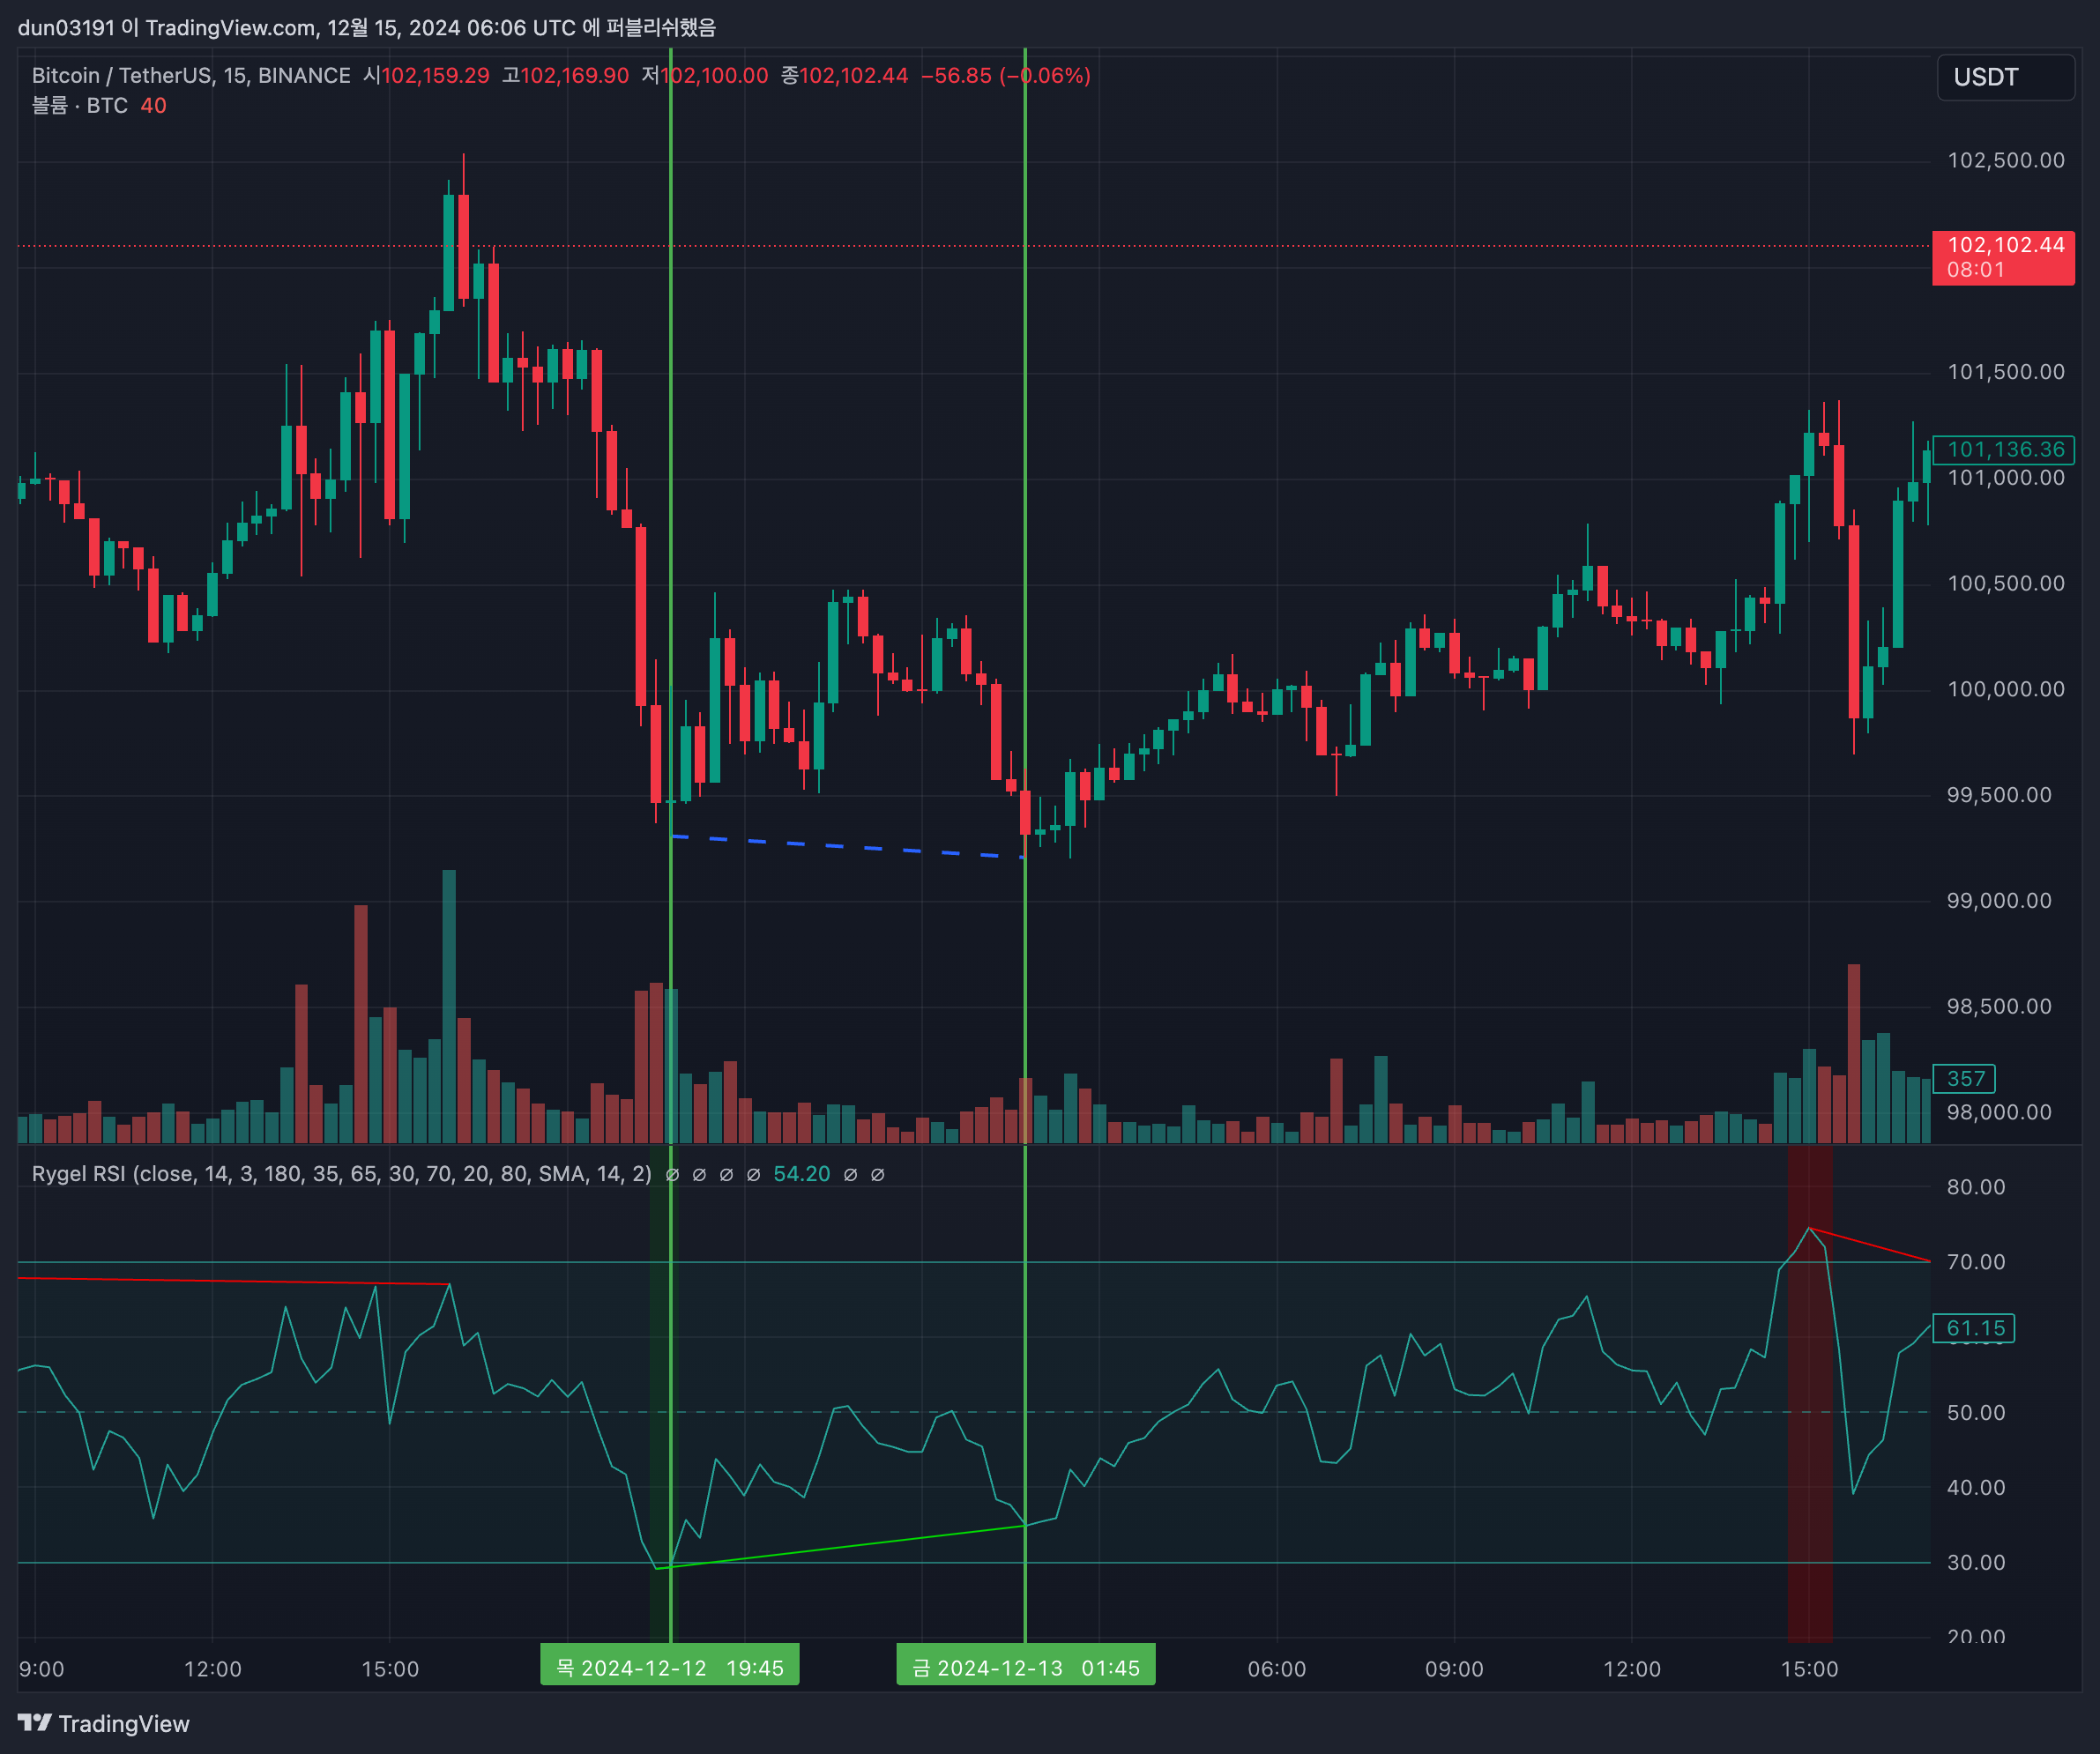
\includegraphics[width=3.0in]{fig1-bullish_divergence.png}
   \caption{An example of a bullish divergence: Price makes a lower low (LL) while RSI makes a higher low (HL). The vertical lines mark the detected divergence window.}
   \label{fig:bullish_div_example}
\end{figure}

\subsection{Calculating TP and SL Levels}
After detecting a divergence, we set:
\begin{itemize}
    \item \textbf{Bullish}: TP at 0.382 Fibonacci retracement from divergence low to previous significant high; SL at the divergence low itself.
    \item \textbf{Bearish}: TP at 0.618 retracement from divergence high to previous significant low; SL at the divergence high.
\end{itemize}

These levels are chosen to reflect common Fibonacci retracements and provide a systematic approach to trade exits.

\subsection{Trade Labeling Procedure}
Once TP and SL are defined, we label each divergence:
\begin{itemize}
    \item Start checking from the divergence end time plus a few bars (to simulate realistic entry).
    \item If price hits TP before SL, label = 1 (True/profitable).
    \item If price hits SL before TP, label = 0 (False/not profitable).
\end{itemize}

This labeling ensures a binary classification task: Given the past sequence and divergence conditions, predict if this signal would have been profitable.

%%%%%%%%%%%%%%%%%%%%%%%%%%%%%%%%%%%%%%%%%%%%%%%%%%%%%%%%%%%%%%%%%%%%%%%%%%%%%%%%
\section{MODEL ARCHITECTURES AND TRAINING}

\subsection{LSTM-Based Model}
We first implement a baseline LSTM model:
\begin{itemize}
    \item Input: A sequence of length $L$ (e.g., $L=288$ bars, corresponding to about one day of 5m data).
    \item LSTM Layers: 1--2 layers, each with 64--128 hidden units.
    \item Final Hidden State: Concatenated with non-sequential features (divergence type, TP\_percent, SL\_percent, multi-timeframe divergence flags).
    \item Fully-Connected Layers: One or two FC layers (e.g., 64 hidden units) with ReLU activations leading to a final sigmoid output for binary classification.
\end{itemize}

\subsection{Transformer-Based Model}
We replace LSTM with a Transformer encoder:
\begin{itemize}
    \item Input Projection: Map input features ($\sim$24 features) to a model dimension $d_{model}$ (e.g., 128--256).
    \item Positional Encoding: Add positional embeddings to reflect temporal order.
    \item Transformer Encoders: 2--4 layers, each with 4--8 attention heads, feedforward dimension of $4 \times d_{model}$, dropout=0.1--0.3.
    \item Pooling: Mean-pool the final encoded sequence or use a learnable [CLS] token representation.
    \item Concatenate Pooled Vector with Non-Sequential Features: Feed into a small MLP (64--128 units) and output a binary class.
\end{itemize}

Transformers often capture long-range dependencies more effectively, potentially extracting subtle divergence signals better than LSTMs.

\subsection{Training Details}
\begin{itemize}
    \item Loss: Binary Cross-Entropy with class weights.
    \item Optimizer: AdamW with learning rate 1e-3 to 1e-4, weight decay for regularization.
    \item Early Stopping: Monitor validation loss or accuracy; patience of 50 epochs.
    \item Batch Size: 64.
\end{itemize}

We also consider using techniques like Focal Loss if the model tends to predict all zeros. Hyperparameter search (learning rates, hidden sizes, number of layers) further refines the model.

%%%%%%%%%%%%%%%%%%%%%%%%%%%%%%%%%%%%%%%%%%%%%%%%%%%%%%%%%%%%%%%%%%%%%%%%%%%%%%%%
\section{Results and Analysis}

\subsection{Evaluation Metrics}
The following metrics are used to evaluate model performance:
\begin{itemize}
    \item \textbf{Accuracy}: The percentage of correctly classified signals.
    \item \textbf{Precision} and \textbf{Recall}: Useful for analyzing performance on imbalanced datasets.
    \item \textbf{F1-Score}: The harmonic mean of precision and recall, balancing their trade-off.
\end{itemize}

\subsection{Preliminary Results}
Initial experiments reveal the following:
\begin{itemize}
    \item Introducing class weights increases the LSTM accuracy to approximately 70\%.
    \item The Transformer model, with careful hyperparameter tuning (e.g., $d_{model}=256$, 2 encoder layers, 8 attention heads), achieves an accuracy of 74\%. However, the recall remains extremely low (0.004), indicating that the model predicts almost all samples as class 0 (Non-Profit). Detailed results are provided in Table~\ref{table:model_performance}.
\end{itemize}

\begin{table}[h]
\caption{Model Performance Comparison}
\label{table:model_performance}
\centering
\begin{tabular}{lccc}
\toprule
\textbf{Model} & \textbf{Accuracy} & \textbf{Precision} & \textbf{Recall} \\
\midrule
LSTM (with class weights) & 0.70 & 0.00 & 0.00 \\
Transformer (tuned) & 0.74 & 0.50 & 0.004 \\
\bottomrule
\end{tabular}
\end{table}

\subsection{Confusion Matrix}
The confusion matrix in Table~\ref{table:confusion_matrix} illustrates the Transformer model's performance. It shows that most of the samples are predicted as class 0 (Non-Profit), confirming the recall issue.

\begin{table}[h!]
\caption{Confusion Matrix of Transformer Model}
\label{table:confusion_matrix}
\centering
\begin{tabular}{|c|c|c|}
\hline
\textbf{True Label} & \textbf{Predicted: Non-Profit (0)} & \textbf{Predicted: Profit (1)} \\ \hline
\textbf{Non-Profit (0)} & 616 & 1 \\ \hline
\textbf{Profit (1)} & 213 & 1 \\ \hline
\end{tabular}
\end{table}

\subsection{Training Convergence}
Figure~\ref{fig:training_loss_transformer} shows the training and validation loss for the Transformer model across epochs. Although the model converges during training, its performance on validation data indicates significant room for improvement.

\begin{figure}[h]
    \centering
    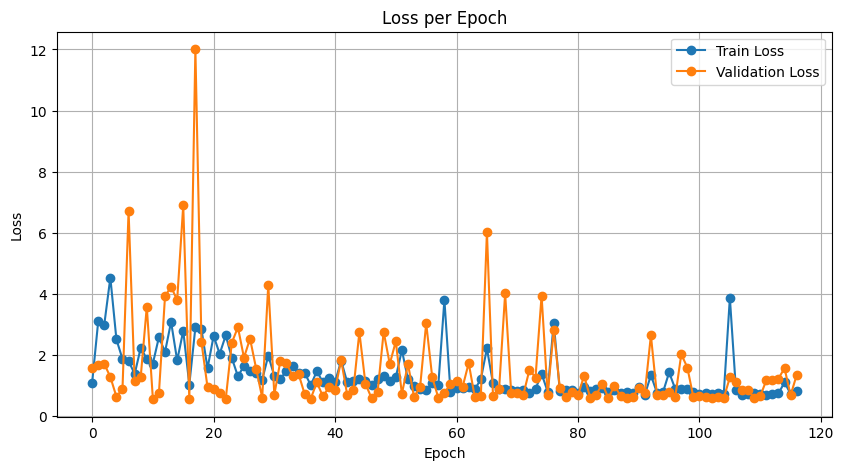
\includegraphics[width=3.0in]{fig2-trasnformer_epoch.png}
    \caption{Training and validation loss during Transformer model training.}
    \label{fig:training_loss_transformer}
\end{figure}

%%%%%%%%%%%%%%%%%%%%%%%%%%%%%%%%%%%%%%%%%%%%%%%%%%%%%%%%%%%%%%%%%%%%%%%%%%%%%%%%
\section{Discussion and Future Study}

In this study, we attempted to train both LSTM and Transformer models for classifying the divergence data, but both models exhibited a tendency to predict all the validation and test data as non-profit (label: 0). Despite trying various methods, such as adjusting the number of layers, refining the vector size, changing the optimizer, and modifying the learning rate, we were unable to significantly improve the model’s performance. This indicates that there might be other underlying issues with the data or model architecture that need to be addressed.

\subsection{Limitations}
\begin{itemize}
    \item The primary limitation of this study is the dataset itself, particularly the presence of repeated or near-identical sequences. This redundancy might have caused the model to struggle in differentiating between sequences, leading to suboptimal performance.
    \item The imbalance in the dataset, with a higher proportion of non-profit labels, could have biased the model towards predicting the majority class, as it failed to learn from the minority class effectively.
    \item Despite extensive tuning of hyperparameters and model architecture, we could not achieve a substantial improvement in model performance, suggesting that other aspects of the data or features might need further investigation.
\end{itemize}

\subsection{Future Study}
\begin{itemize}
    \item \textbf{Data Refinement}: A more thorough data cleaning process is required to identify and remove duplicate or nearly identical sequences, especially those with the same start time but different end times. This would help reduce redundancy and potentially improve the model’s ability to generalize.
    \item \textbf{Feature Engineering}: Future work should focus on refining the features used in the model. For example, more advanced feature extraction techniques or transformations could be applied to better capture the underlying patterns in the data. Techniques such as normalization, scaling, or more sophisticated methods of combining technical indicators (RSI, MACD) could be explored.
    \item \textbf{Addressing Class Imbalance}: One possible solution for dealing with the class imbalance issue is to use resampling methods, such as oversampling the minority class or undersampling the majority class, or employing more advanced techniques like focal loss to prioritize the minority class.
    \item \textbf{Model Improvements}: Exploring more complex models or hybrid approaches could be another avenue for future research. For instance, integrating convolutional layers with LSTM or Transformer architectures might help capture more localized patterns in the data, which could improve the classification task.
    \item \textbf{Model Interpretability}: It would be valuable to investigate model interpretability techniques, such as SHAP values or permutation importance, to better understand which features are most influential in the model’s decision-making process. This could provide insights into the underlying mechanisms and improve model tuning.
\end{itemize}

%%%%%%%%%%%%%%%%%%%%%%%%%%%%%%%%%%%%%%%%%%%%%%%%%%%%%%%%%%%%%%%%%%%%%%%%%%%%%%%%
\section{CONCLUSIONS}

In this study, we proposed a systematic approach to detect RSI divergences and classify trade opportunities as profitable or non-profitable. By combining an effective divergence detection algorithm with a well-defined trade labeling schema (using TP and SL levels) and integrating a broad range of technical features, we created a dataset well-suited for training advanced time-series models.

Our results highlight the following key findings:
\begin{itemize}
    \item Data processing for RSI divergence data has been made, providing a structured foundation for model training.
    \item Proper handling of class imbalance and thoughtful feature engineering are critical to improving model performance.
    \item Transformer models are more effective than LSTM models in capturing the nuanced temporal dependencies present in divergence patterns.
    \item Evaluation metrics, such as confusion matrices, are valuable tools for understanding model behavior and identifying areas for further refinement.
\end{itemize}

Future work will explore alternative exit strategies, the inclusion of sentiment and macroeconomic indicators, and the testing of more advanced architectures and regularization techniques to further enhance model robustness and predictive performance.

%%%%%%%%%%%%%%%%%%%%%%%%%%%%%%%%%%%%%%%%%%%%%%%%%%%%%%%%%%%%%%%%%%%%%%%%%%%%%%%%
\begin{thebibliography}{99}

\bibitem{c1} J. Murphy, \textit{Technical Analysis of the Financial Markets}, New York Institute of Finance, 1999.
\bibitem{c2} A. Elder, \textit{Trading for a Living: Psychology, Trading Tactics, Money Management}, John Wiley \& Sons, 1993.
\bibitem{c3} S. Hochreiter and J. Schmidhuber, ``Long Short-Term Memory,'' \textit{Neural Computation}, vol. 9, no. 8, 1997.
\bibitem{c4} A. Vaswani et al., ``Attention Is All You Need,'' \textit{NIPS}, 2017.
\bibitem{c5} T. Chen et al., ``A Gentle Introduction to Long-Term Dependence in Time Series,'' {\it arXiv preprint arXiv:xxxx.xxxx}, 2020.
\bibitem{c6} M. F. Dixon, I. Halperin, and P. Bilokon, {\it Machine Learning in Finance}, Springer, 2020.

\end{thebibliography}

\end{document}
